\section{Datos, depuración de cohorte y análisis exploratorio}\label{sec:datos_eda}

Antes de formular los conjuntos experimentales o el estimador, esta sección caracteriza las fuentes de datos, las reglas de depuración física con sus posibles sesgos de selección, y la evidencia exploratoria que motiva cada decisión de modelado.

\subsection{Fuentes de información y depuración causal de la cohorte}

La base empírica cubre el periodo comprendido entre el 1 de enero de 2024 y el 31 de octubre de 2026 ($1\,035$ días calendario) e integra cuatro fuentes auditadas: (1) generación horaria real medida y capacidad efectiva neta diaria reportadas por el operador del mercado eléctrico colombiano XM \cite{xm2026api}; (2) coordenadas geográficas verificadas de las centrales en el \textit{Global Solar Power Tracker} \cite{gem2026solar}; (3) pronósticos meteorológicos horarios a $24\text{ h}$ de antelación (promedio del ensamble ECMWF IFS $0{,}25^\circ$, GFS e ICON) recuperados de los archivos históricos de la API \textit{Previous Runs} de Open-Meteo \cite{openmeteoPreviousRuns}; y (4) corridas operacionales subestacionales del sistema NOAA GEFSv12 (\texttt{00~UTC}, pasos horarios hasta $696\text{ h}$, equivalentes a $29$ días), totalizando $65\,688$ registros completos planta--origen--horizonte. Durante la auditoría inicial se descartó reconstruir pronósticos históricos $D+1$ a partir de las primeras horas de las corridas de archivo, pues su elevada proximidad al reanálisis meteorológico (correlación $0{,}976$ frente a $0{,}615$ del pronóstico real emitido con $24\text{ h}$ de antelación) habría introducido fuga de información futura.

El protocolo de depuración física \cite{nist2003eda,pipino2002quality,jensen2024solarqc} parte de $30\,964$ registros recurso--día de XM y aplica filtros secuenciales estrictos: existencia de capacidad efectiva neta registrada en la fecha, generación y capacidad estrictamente positivas, plausibilidad física $\mathrm{cf}^{\mathrm{obs}}_{i,t} \le 1{,}05$ (admitiendo un margen de $5\%$ para tolerar pequeñas diferencias horarias antes de reportar ampliaciones), coordenadas verificadas, al menos $60$ días transcurridos desde la entrada en operación comercial y un mínimo de $100$ días útiles por planta. La Figura~\ref{fig:cohorte_mapa} resume el flujo cuantitativo de depuración hasta consolidar $12\,756$ observaciones planta--día en $M=17$ centrales distribuidas en $G=7$ zonas geográficas (agrupadas por enlace simple a menos de $100\text{ km}$). Para el ajuste y evaluación causal se exige además contar con más de $6$ horas reportadas en el día, excluyendo $31$ registros incompletos ($0{,}24\%$, todos con factor de capacidad inferior a $0{,}04$) hasta obtener $12\,725$ días válidos, sin imputar jamás la variable objetivo.

\begin{figure}[!htbp]
\centering
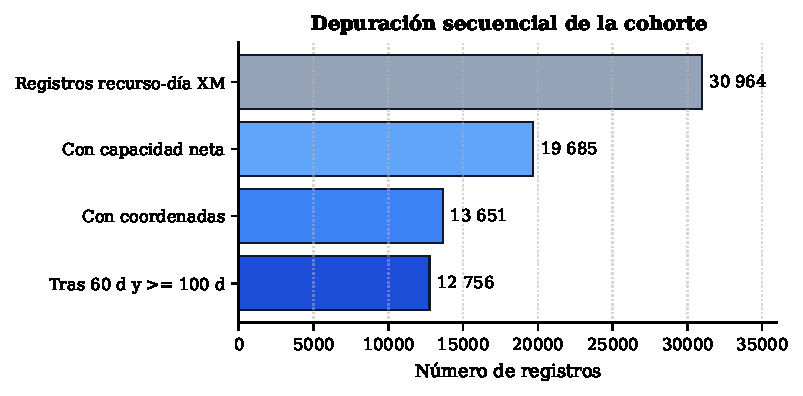
\includegraphics[width=0.86\textwidth]{figures/eda_flujo_cohorte.pdf}\\[0.5em]
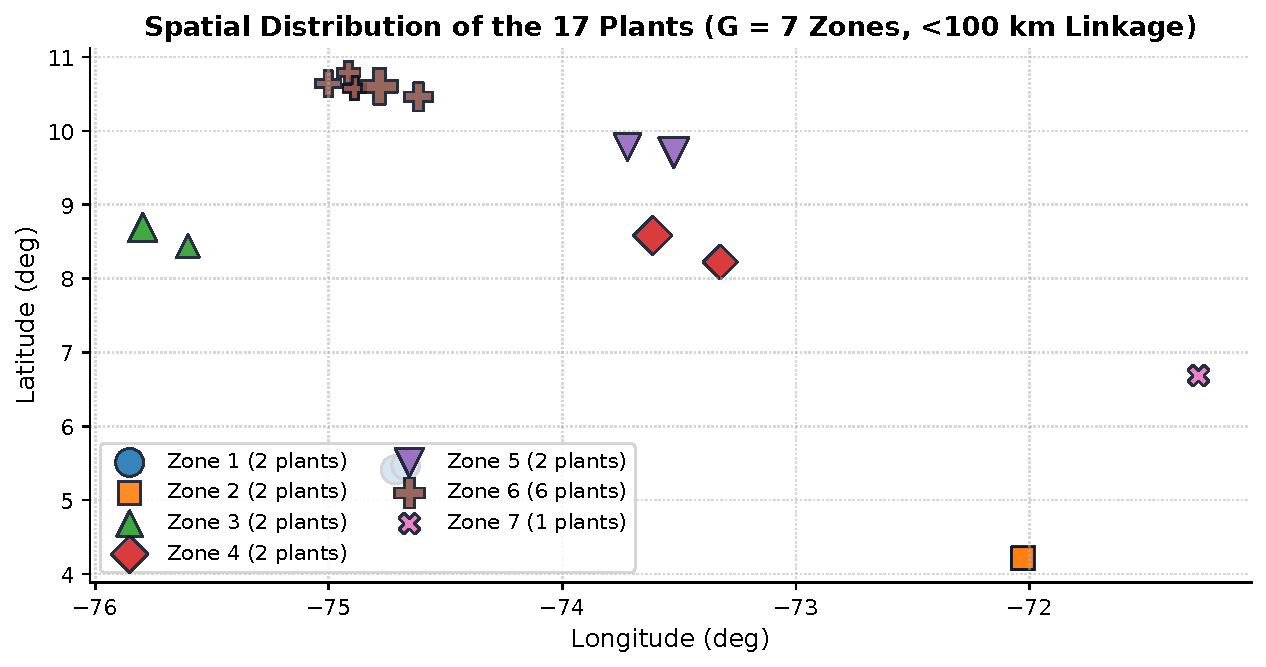
\includegraphics[width=0.86\textwidth]{figures/eda_mapa_plantas.pdf}
\caption{Depuración cuantitativa de la cohorte ($30\,964 \to 12\,756$ registros planta--día en $17$ centrales; arriba) y distribución geográfica en $G=7$ zonas espaciales por enlace simple a $<100\text{ km}$ (abajo).}
\label{fig:cohorte_mapa}
\end{figure}

Es indispensable explicitar los posibles sesgos de selección derivados de estos filtros: al excluir días con generación nula o $\le 6$ horas reportadas, las métricas reflejan operación activa o parcialmente activa y omiten paradas totales prolongadas; asimismo, el requisito de $\ge 100$ días útiles y $\ge 60$ días post-arranque excluye plantas recién conectadas en fase temprana de pruebas, concentrando la muestra en centrales operativamente estabilizadas cuya cobertura oscila entre $251$ y $1\,032$ días válidos (Tabla~\ref{tab:flota17}).

\begin{table}[!htbp]
\caption{Caracterización de las $17$ centrales fotovoltaicas de la cohorte (ordenadas por grupo espacial).}\label{tab:flota17}
\scriptsize
\setlength{\tabcolsep}{3.5pt}
\begin{tabular}{@{}clrrrrrr@{}}
\toprule
Cód. & Planta & Gr. & $n$ total & Cap.\ mín--máx (MW) & Inicio & Fin & Lat / Lon ($^\circ$) \\
\midrule
\texttt{3IRX} & Portón del Sol & 1 & 884 & $102{,}0$--$102{,}0$ & 2024-05-07 & 2026-10-31 & $5{,}41 / -74{,}71$ \\
\texttt{TPUY} & Parque Solar Tepuy & 1 & 812 & $83{,}0$--$100{,}0$ & 2024-08-11 & 2026-10-31 & $5{,}47 / -74{,}67$ \\
\texttt{3EDL} & Bosques Llanos V & 2 & 1\,034 & $17{,}9$--$17{,}9$ & 2024-01-01 & 2026-10-31 & $4{,}21 / -72{,}03$ \\
\texttt{3EFY} & Bosques Llanos IV & 2 & 1\,034 & $19{,}9$--$19{,}9$ & 2024-01-01 & 2026-10-31 & $4{,}22 / -72{,}03$ \\
\texttt{3IZ6} & Parque Solar La Unión & 3 & 805 & $100{,}0$--$102{,}0$ & 2024-08-18 & 2026-10-31 & $8{,}69 / -75{,}80$ \\
\texttt{3J2B} & Solar Planeta Rica & 3 & 868 & $19{,}9$--$19{,}9$ & 2024-06-16 & 2026-10-31 & $8{,}44 / -75{,}60$ \\
\texttt{3IQA} & Sunnorte & 4 & 643 & $35{,}0$--$35{,}0$ & 2025-01-25 & 2026-10-31 & $8{,}22 / -73{,}32$ \\
\texttt{MATA} & La Mata & 4 & 796 & $80{,}0$--$83{,}0$ & 2024-08-26 & 2026-10-31 & $8{,}59 / -73{,}61$ \\
\texttt{3DDT} & Latam Solar La Loma & 5 & 795 & $150{,}0$--$150{,}0$ & 2024-08-23 & 2026-10-31 & $9{,}71 / -73{,}52$ \\
\texttt{EPFV} & El Paso & 5 & 892 & $68{,}0$--$70{,}0$ & 2024-05-22 & 2026-10-31 & $9{,}78 / -73{,}72$ \\
\texttt{3HF5} & Fundación & 6 & 800 & $90{,}0$--$100{,}0$ & 2024-08-21 & 2026-10-31 & $10{,}46 / -74{,}62$ \\
\texttt{3INX} & Caracolí I & 6 & 618 & $50{,}0$--$50{,}0$ & 2025-02-20 & 2026-10-31 & $10{,}64 / -75{,}00$ \\
\texttt{3K8C} & BSB 503 & 6 & 699 & $19{,}9$--$19{,}9$ & 2024-11-25 & 2026-10-31 & $10{,}57 / -74{,}89$ \\
\texttt{3K8E} & BSB 504 & 6 & 698 & $19{,}9$--$19{,}9$ & 2024-11-26 & 2026-10-31 & $10{,}58 / -74{,}89$ \\
\texttt{4RGG} & Parque Solar Baranoa & 6 & 490 & $19{,}9$--$19{,}9$ & 2025-06-29 & 2026-10-31 & $10{,}79 / -74{,}92$ \\
\texttt{GYPO} & Guayepo & 6 & 635 & $370{,}0$--$388{,}0$ & 2025-01-29 & 2026-10-31 & $10{,}61 / -74{,}78$ \\
\texttt{5F43} & Alma II & 7 & 253 & $9{,}8$--$9{,}8$ & 2026-02-21 & 2026-10-31 & $6{,}69 / -71{,}28$ \\
\botrule
\end{tabular}
\end{table}

\subsection{Hallazgos exploratorios y su vínculo con el diseño del estimador}

Cada figura exploratoria responde una pregunta científica específica que condiciona las decisiones metodológicas posteriores:

\paragraph{1. ¿Qué heterogeneidad de cobertura, escala y ampliaciones presenta la flota?}
La Tabla~\ref{tab:flota17} y la Figura~\ref{fig:eda_cob_horas} muestran que las centrales entran en operación de forma escalonada (desde enero de 2024 hasta febrero de 2026), con capacidades netas entre $9{,}8$~MW (\texttt{5F43}) y $388{,}0$~MW (\texttt{GYPO}), un cociente de escala de $39{,}6\times$, y $7$ ampliaciones discretas de potencia neta en $6$ centrales (por ejemplo, \texttt{TPUY} de $83$ a $100$~MW y \texttt{3HF5} de $90$ a $100$~MW). Asimismo, la distribución de horas reportadas confirma la presencia de $31$ jornadas truncadas ($\le 6\text{ h}$) asociadas a valores anormalmente bajos. Estas dos observaciones justifican tres decisiones: (a) normalizar tanto predictores históricos como objetivos en factor de capacidad usando exclusivamente la capacidad vigente al origen $C_{i,t}$ sin anticipar ampliaciones futuras; (b) agregar errores mediante macro-promedio por planta ($\mathrm{MAE}_{\mathrm{macro}}$) para no quedar dominados por las plantas de mayor potencia o mayor longitud de serie; y (c) excluir días incompletos de $\le 6\text{ h}$ para no contaminar la señal física con fallas de telemetría.

\begin{figure}[!htbp]
\centering
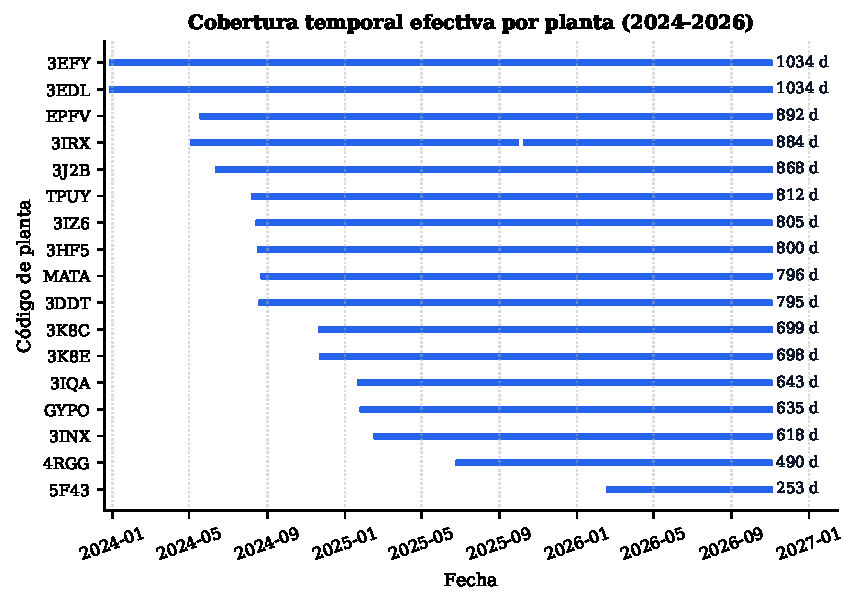
\includegraphics[width=0.92\textwidth]{figures/eda_cobertura_temporal.pdf}\\[0.5em]
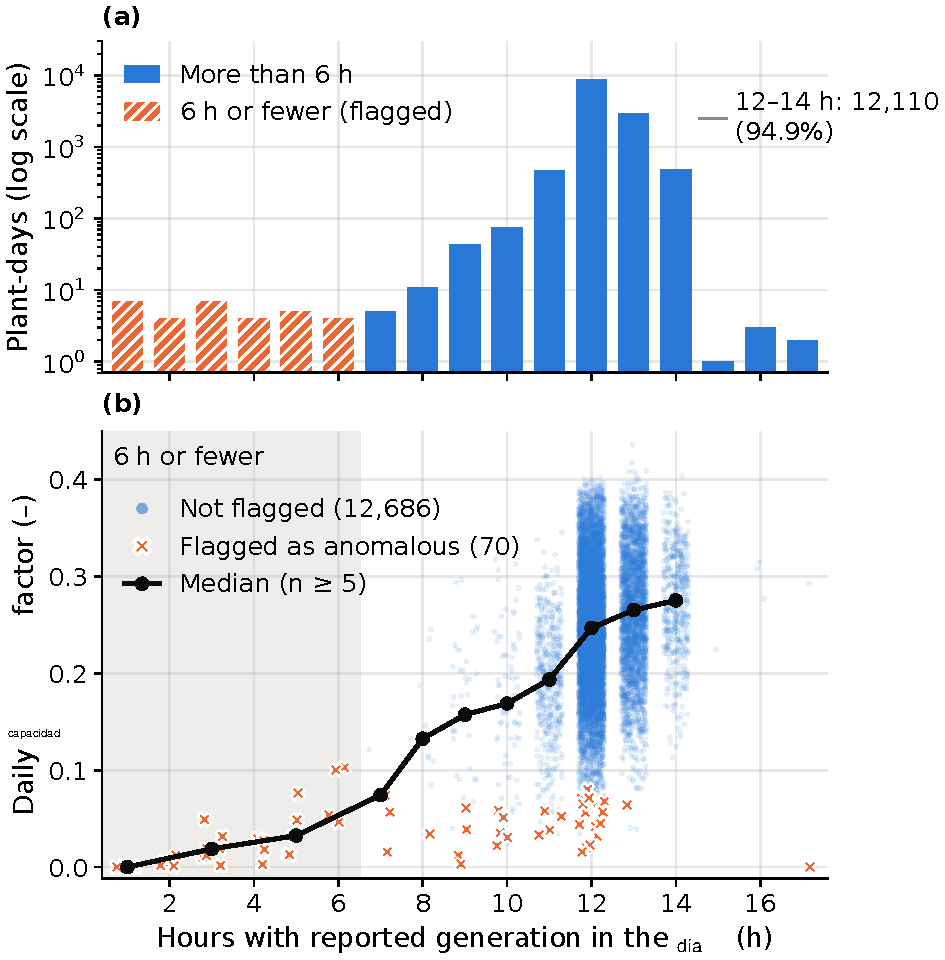
\includegraphics[width=0.92\textwidth]{figures/eda_horas_y_anomalos.pdf}
\caption{Cobertura temporal heterogénea por planta ($251$ a $1\,032$ días útiles; arriba) y distribución de horas reportadas por XM mostrando los registros incompletos excluidos ($\le 6\text{ h}$; abajo).}
\label{fig:eda_cob_horas}
\end{figure}

\paragraph{2. ¿Cómo se distribuyen el factor de capacidad y la relación con la irradiación?}
La Figura~\ref{fig:eda_univ} muestra que el factor de capacidad diario observado posee media $0{,}248$, mediana $0{,}250$ (rango intercuartílico $0{,}203$--$0{,}295$; máximo $0{,}436$) y una cola izquierda extendida hacia cero. Al graficarlo frente a la irradiación horizontal diaria pronosticada, se observa una asociación positiva monótona acompañada de $68$ episodios de rendimiento específico reducido (cociente entre factor de capacidad normalizado e irradiación inferior a $0{,}3$). Sin registros independientes de consignas de despacho no puede atribuirse la totalidad de esos episodios a \textit{curtailment}: reflejan una mezcla de restricciones operativas, desconexiones parciales, mantenimiento y nubosidad convectiva local no capturada por la malla NWP. Desde el punto de vista metodológico, esta evidencia motiva evaluar la pérdida de Huber con escalado robusto MAD para acotar el peso de caídas anómalas en la respuesta, junto con restricciones de signo no negativo sobre la irradiación pronosticada y la persistencia reciente para evitar pendientes negativas espurias.

\begin{figure}[!htbp]
\centering
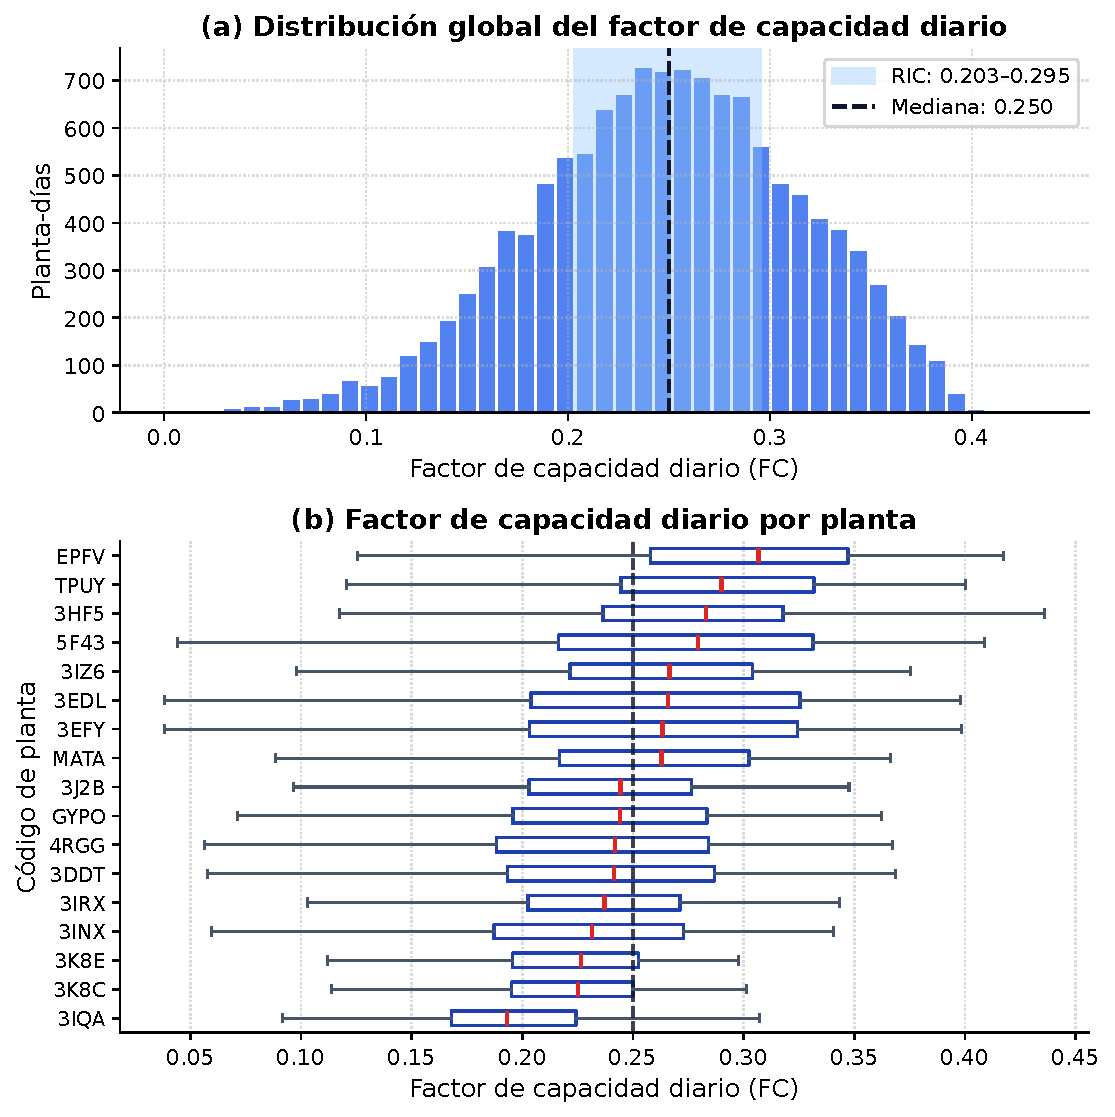
\includegraphics[width=0.49\textwidth]{figures/eda_distribucion_fc.pdf}
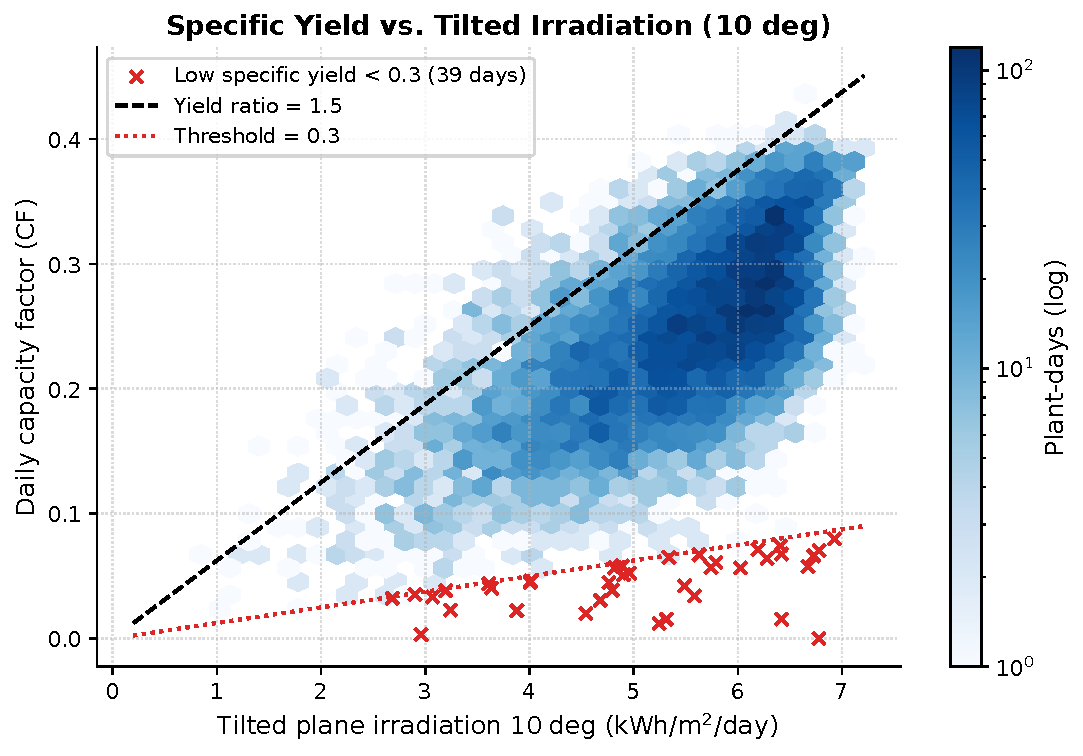
\includegraphics[width=0.49\textwidth]{figures/eda_rendimiento_especifico.pdf}
\caption{Distribución asimétrica del factor de capacidad diario observado (izquierda) y relación empírica frente a la irradiación diaria destacando $68$ episodios de rendimiento específico reducido (derecha).}
\label{fig:eda_univ}
\end{figure}

\paragraph{3. ¿Qué estructura de estacionalidad, persistencia y acoplamiento espacial existe?}
La Figura~\ref{fig:eda_est_dep} evidencia una variación mensual moderada acorde con los ciclos climáticos de Colombia (regiones Caribe, Andina y Orinoquía), una autocorrelación positiva pronunciada en rezagos cortos que decae progresivamente con el tiempo, y correlaciones cruzadas significativas entre plantas pertenecientes a la misma zona geográfica ($<100\text{ km}$). La persistencia temporal fundamenta incluir medias móviles causales de $30$ y $7$ días junto con diferencias amortiguadas por horizonte y armónicos anuales de calendario; a su vez, la elevada correlación intrazonal demuestra que una validación espacial ingenua por planta individual filtraría información de centrales vecinas situadas en el mismo régimen nuboso, haciendo obligatoria la validación \textit{leave-one-group-out} por conglomerados de $<100\text{ km}$ y la inferencia robusta con varianza HAC.

\begin{figure}[!htbp]
\centering
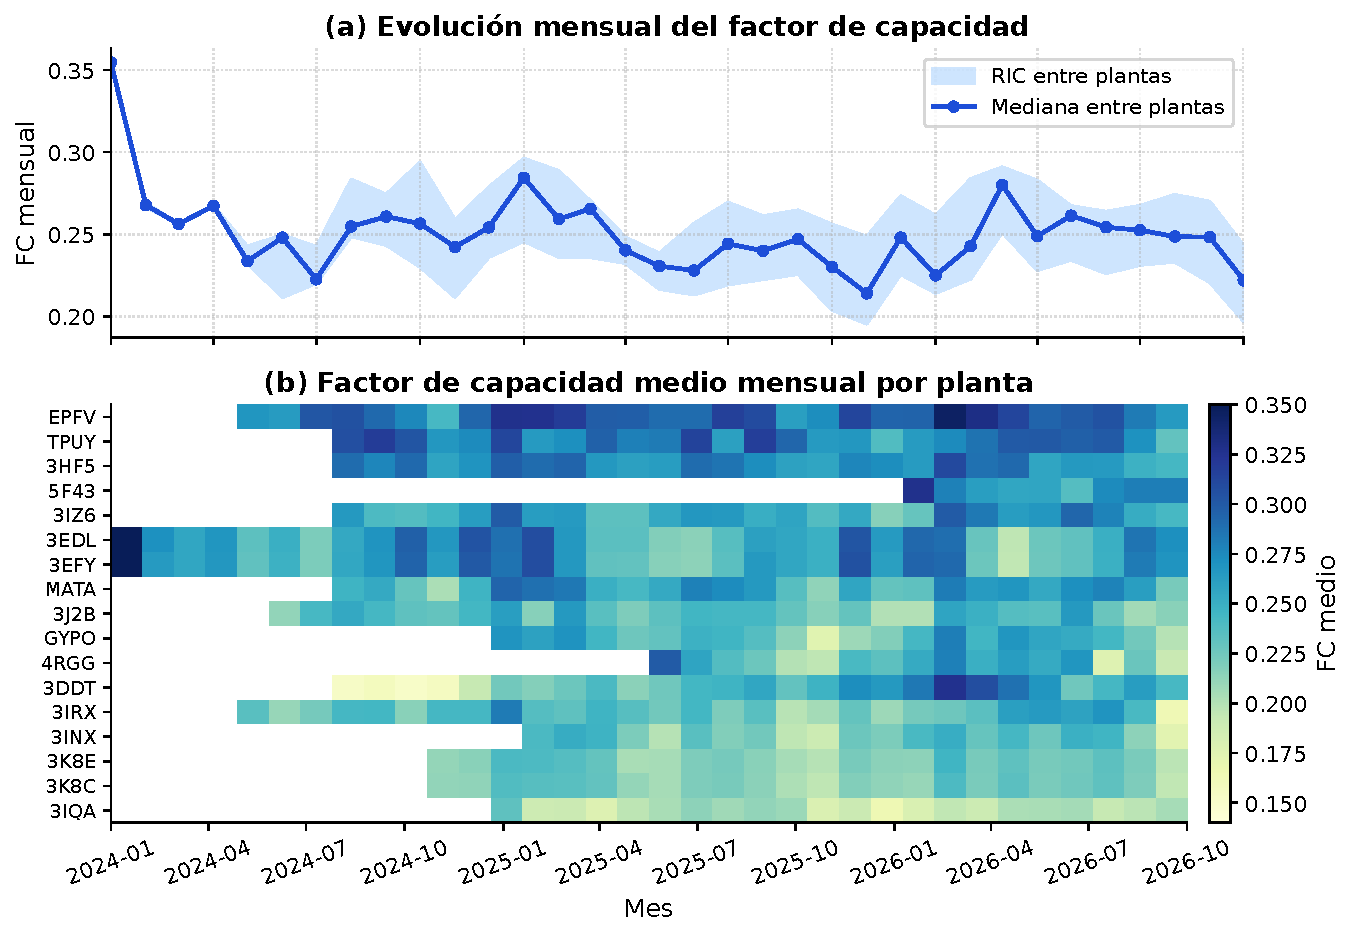
\includegraphics[width=0.92\textwidth]{figures/eda_estacionalidad.pdf}\\[0.5em]
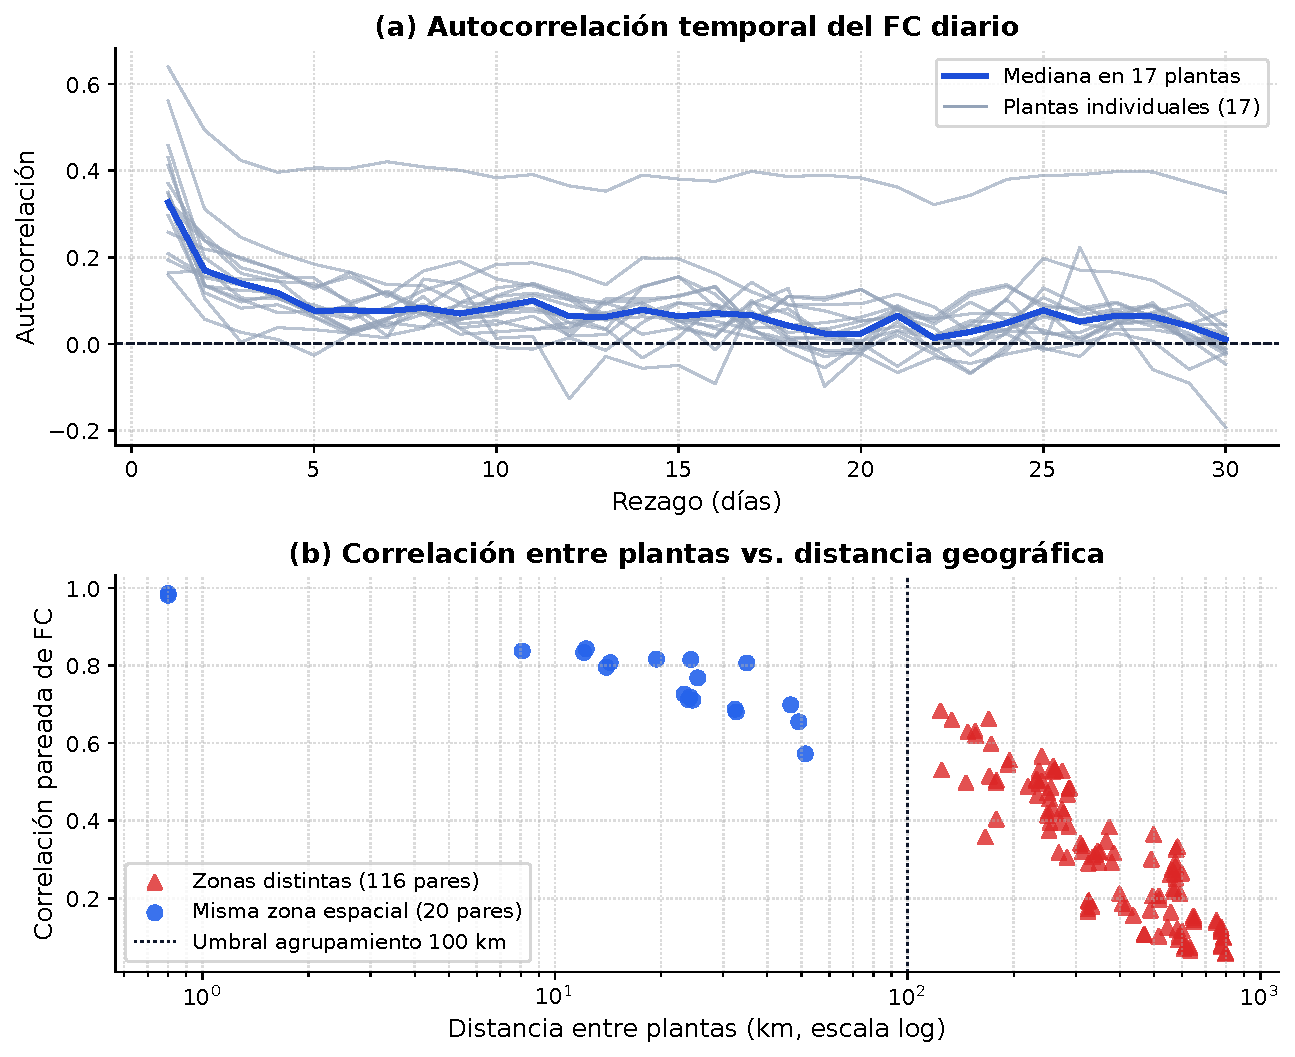
\includegraphics[width=0.92\textwidth]{figures/eda_dependencia.pdf}
\caption{Estacionalidad mensual del factor de capacidad (arriba) y estructura de autocorrelación temporal y correlación espacial entre centrales (abajo).}
\label{fig:eda_est_dep}
\end{figure}

\paragraph{4. ¿Qué comportamiento presentan las variables meteorológicas pronosticadas?}
Finalmente, la Figura~\ref{fig:eda_clima} muestra la distribución y dinámica de las cinco variables meteorológicas pronosticadas sobre la cohorte (irradiación horizontal, temperatura a $2\text{ m}$, nubosidad total, humedad relativa y velocidad del viento a $10\text{ m}$). La dispersión regional y la variabilidad atmosférica motivan complementar los niveles NWP absolutos con anomalías causales respecto a la media móvil reciente de $30$ días de cada planta y asignar una regularización cuadrática diferenciada ($\alpha_{\mathrm{meteo}}$) capaz de atenuar su influencia cuando la habilidad NWP se degrada en horizontes subestacionales.

\begin{figure}[!htbp]
\centering
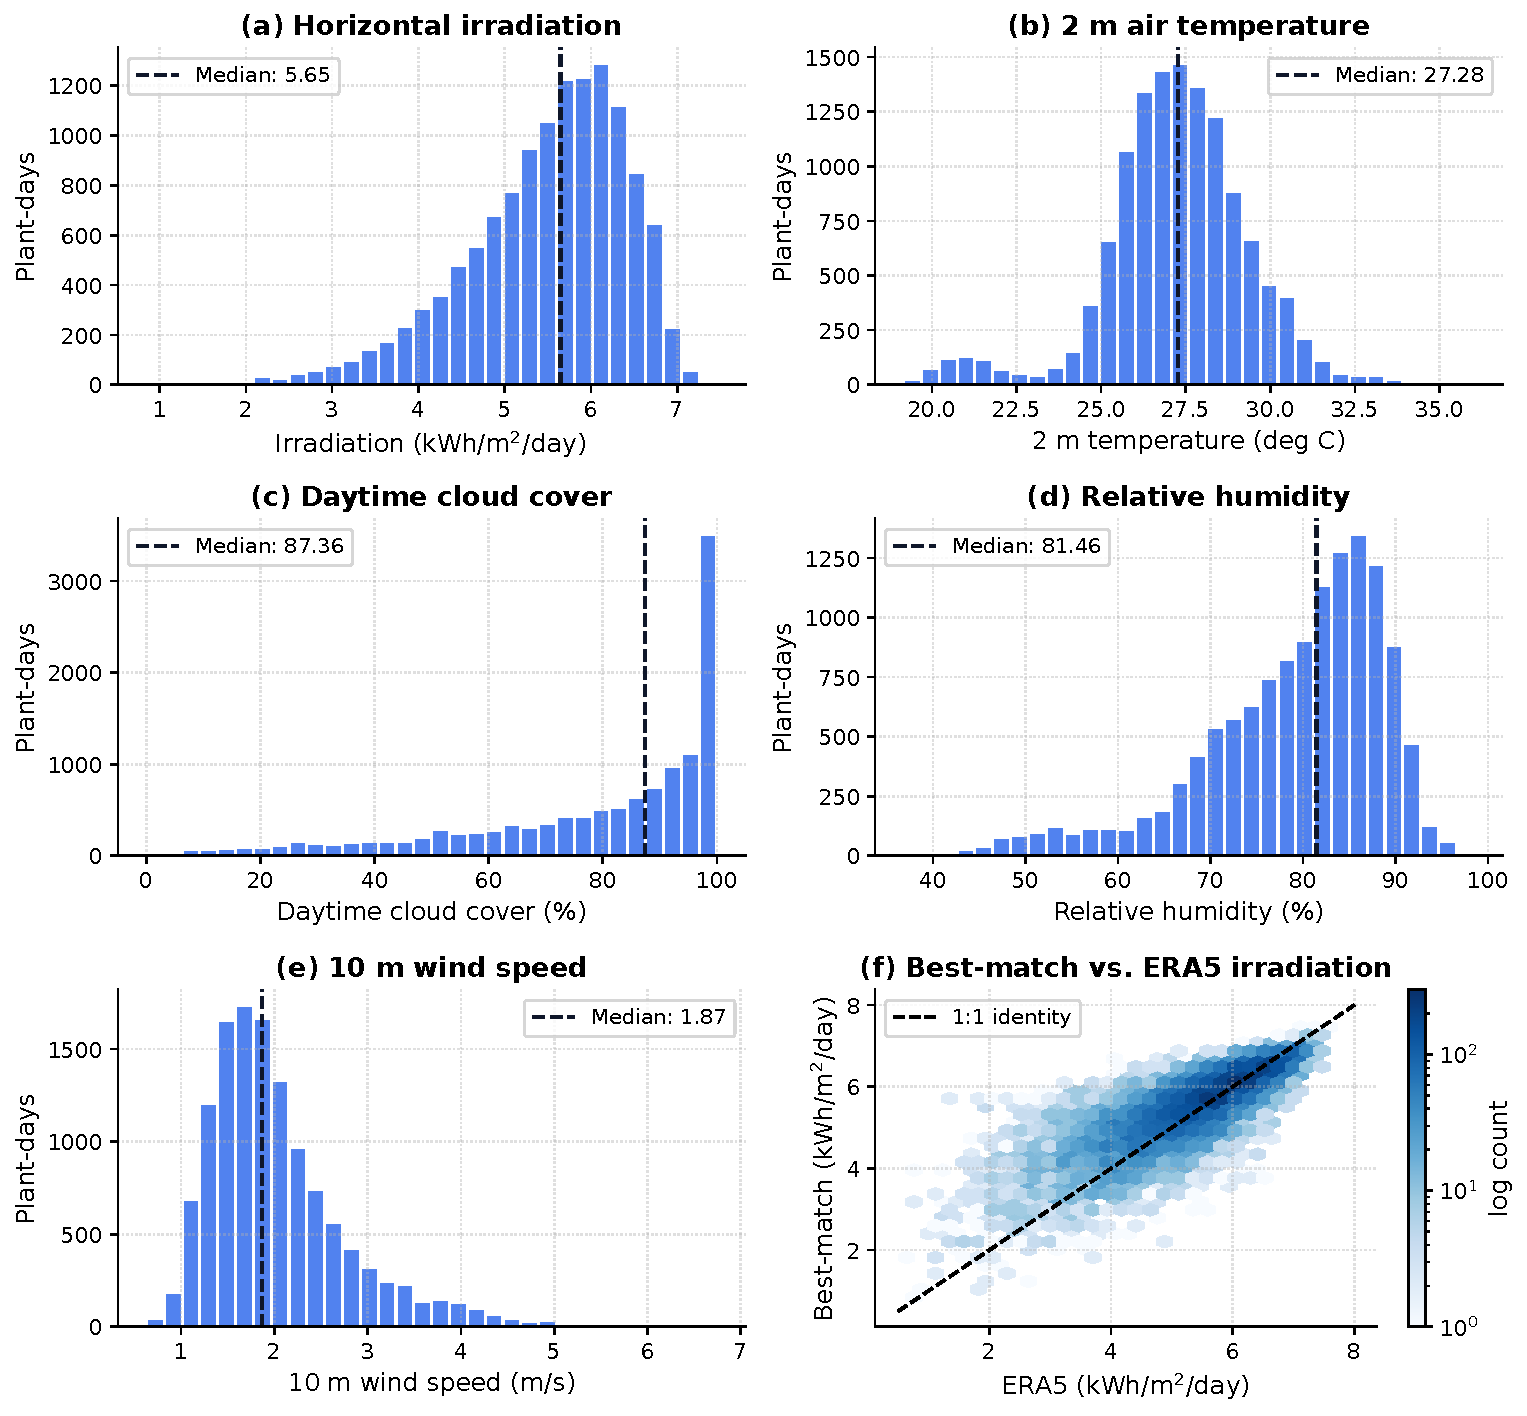
\includegraphics[width=0.92\textwidth]{figures/eda_clima.pdf}
\caption{Distribución y dinámica de las cinco variables meteorológicas pronosticadas sobre la cohorte de $17$ centrales.}
\label{fig:eda_clima}
\end{figure}
